% Provenance (never printed): see sources/outline_sources.md (Year 3:
% moments of inertia and gravity fields; impact cratering and crater dating;
% volcanism and tectonics on Mars, Venus, Io and the icy moons).
% Brief: sources/book5/BRIEFS.md, ch. 26. Curves from figdata/bachelor-3/
% two_layer_planet.py (two-layer interiors of the Earth, Mars, the Moon and
% Mercury from mean density and moment of inertia) and crater_sfd.py
% (the Ivanov production function and the Hartmann-Neukum chronology of
% Mars from the Craterstats configuration, the lunar chronology of Neukum,
% Hartmann's equilibrium density, and two invented Martian plains whose
% counts are drawn once from a Poisson law). Exercise and problem values in
% the Book 5 scratch calculator calc/ch26.py. Plains A and B are invented.
\chapter{Planetaire binnenwerelden en oppervlakken}\label{ch:b3:planetary-interiors-surfaces}

Door een verrekijker gezien heeft de Maan twee soorten bodem. De lichte
hooglanden zitten vol kraters, krater op krater: ze zijn
met grote kraters verzadigd door een hevig bombardement dat ongeveer 3.8 miljard
jaar geleden eindigde. De donkere maria, vlakten die tussen 4.2 en 1.2
miljard jaar geleden met lava gevuld raakten, bevatten er veel minder. De missies van Apollo en Luna
brachten gesteente van beide terug, en hun radiometrische ouderdommen maakten
van de kraterdichtheid op een oppervlak een klok. Die klok dateert nu
vlakten op Mars, Mercurius en de ijzige manen, waarvan nog geen gesteente
is teruggebracht. Dit hoofdstuk leest de binnenwerelden van de planeten af aan hun
zwaartekracht, rotatie en getijden, en daarna hun oppervlakken aan hun kraters,
vulkanen en breuken.
% ledger: french:highlands, nasa:moon-core, marchi:neukum

\begin{recall}
De traagheidsmomentfactor $C = I/MR^2$, het tweelaagsmodel van een planeet
dat daaruit en uit de gemiddelde dichtheid wordt opgebouwd, en de terrestrische en de reuzenplaneten
staan in Boek~3, in het hoofdstuk over vergelijkende
planetologie; mantelpluimen en grote vulkanische provincies, in het hoofdstuk over
hotspots. Planetaire differentiatie en de meteorieten staan in Boek~4,
in het hoofdstuk over planeetvorming. De \omterm{def:b3:gravity-geodesy:j2}{dynamische vormfactor}
$J_2$, de \omterm{thm:b3:gravity-geodesy:maccullagh}{formule van MacCullagh} en de buiging van de lithosfeer staan in dit
deel, in het hoofdstuk over zwaartekracht en geodesie; het \omterm{def:b3:mantle-convection:rayleigh}{Rayleighgetal}, in het
hoofdstuk over mantelconvectie. Getijden, de wetten van Kepler en de elastische
moduli staan in de natuurkundeboeken; de Poissonverdeling, in de
wiskundeboeken.
\end{recall}

\section{Binnenwerelden uit zwaartekracht, rotatie en getijden}\label{sec:b3:planetary-interiors-surfaces:interiors}

De massa van een planeet, uit de baan van een maan of een ruimtevaartuig, geeft
de gemiddelde dichtheid; de precessie van zijn as en zijn $J_2$ geven het
traagheidsmoment. De tweelaagspropositie uit Boek~3 zet de twee
getallen om in een kern, maar pas nadat een manteldichtheid is gekozen: twee
metingen kunnen drie onbekenden niet vastleggen.

\begin{omfigure}
\centering
\begin{tikzpicture}
\begin{axis}[width=0.78\linewidth, height=0.46\linewidth,
  xmin=3000, xmax=16000, ymin=0, ymax=1,
  xlabel={kerndichtheid $\rho_c$ (\unit{kg.m^{-3}})},
  ylabel={kernstraal / planeetstraal $x$},
  tick label style={font=\scriptsize}, label style={font=\small},
  scaled x ticks=false, xtick={4000,6000,8000,10000,12000,14000,16000},
  xticklabels={4000,6000,8000,10\,000,12\,000,14\,000,16\,000}]
\addplot[thick, omDef] table[x=rho_c, y=x] {figdata/out/bachelor-3-two_layer_planet-curve-Earth.dat};
\addplot[thick, red!70!black] table[x=rho_c, y=x] {figdata/out/bachelor-3-two_layer_planet-curve-Mars.dat};
\addplot[thick, black!60, dashed] table[x=rho_c, y=x] {figdata/out/bachelor-3-two_layer_planet-curve-Moon.dat};
\addplot[thick, orange!80!black] table[x=rho_c, y=x] {figdata/out/bachelor-3-two_layer_planet-curve-Mercury.dat};
\addplot[only marks, mark=*, mark size=2pt, black] table[x=rho_c, y=x] {figdata/out/bachelor-3-two_layer_planet-points.dat};
\node[font=\scriptsize, omDef, anchor=south west] at (axis cs:12600,0.55) {Aarde};
\node[font=\scriptsize, red!70!black, anchor=south west] at (axis cs:6600,0.55) {Mars};
\node[font=\scriptsize, black!70, anchor=south west] at (axis cs:11000,0.2) {Maan};
\node[font=\scriptsize, orange!80!black, anchor=south west] at (axis cs:7300,0.83) {Mercurius};
\end{axis}
\end{tikzpicture}
\par\smallskip{\small De tweelaagsmodellen die de gemiddelde dichtheid en de
traagheidsmomentfactor van vier hemellichamen toelaten: elke kromme loopt over de
mogelijke manteldichtheden, waarbij een dichtere mantel een kleinere en dichtere
kern oplevert. De stippen markeren de gemeten kernstralen: die van de Aarde uit
seismologie, die van Mars uit de seismometer van InSight, de binnenkern en vloeibare
schil van de Maan, en die van Mercurius uit het zwaartekrachtveld van het
ruimtevaartuig MESSENGER.}\label{fig:b3:planetary-interiors-surfaces:two-layer}
\end{omfigure}
% ledger: planet:Earth.density, planet:Mars.density, planet:Moon.density, planet:Mercury.density, earth:MoI, nasa:mars, nasa:moon, nasa:mercury, data:prem, jpl:insight-interior, nasa:moon-core, agu:mercury-core

Elke planeet levert een kromme op, geen punt. Voor Mars is de kernstraal van
\qty{1830}{km}, door InSight gemeten, kiest een mantel van \qty{3460}{kg.m^{-3}}
en een kern van \qty{6460}{kg.m^{-3}}. Voor Mercurius is de kern van ongeveer
\qty{2000}{km} in straal vult 82~procent van de straal. De kromme van de Maan is
bijna vlak: haar $C = 0.394$ ligt zo dicht bij $\tfrac25$ dat een kleine kern
van welke dichtheid ook past, en een verandering van $0.001$ in $C$ verschuift de kernstraal
met meer dan een factor twee (zie \cref{exo:b3:planetary-interiors-surfaces:10}).
Zwaartekracht alleen ziet geen kleine kern; de getijden en de seismische golven wel.
% ledger: jpl:insight-interior, agu:mercury-core, nasa:moon

\begin{definition}[Lovegetal]\label{def:b3:planetary-interiors-surfaces:love-number}
Wanneer een getijdenpotentiaal van graad~2 op een planeet werkt, vervormt de planeet en
de herverdeelde massa voegt een eigen potentiaal toe. Het
\emph{Lovegetal}\index{Lovegetal} $k_2$ is de verhouding van die toegevoegde potentiaal tot de
getijdenpotentiaal, beide genomen aan het oppervlak van de planeet.
\end{definition}

Een starre planeet heeft $k_2 = 0$; een vloeibare planeet van uniforme dichtheid geeft
volledig mee, met $k_2 = \tfrac32$. Daartussen meet het getal hoeveel van de
planeet meegeeft.

\begin{proposition}[Lovegetal van een uniforme elastische bol]\label{prop:b3:planetary-interiors-surfaces:kelvin}
Een onsamendrukbare bol van uniforme dichtheid $\rho$, straal $R$, oppervlaktezwaartekracht
$g$ en stijfheid $\mu$ heeft
\[
  k_2 = \frac{3/2}{1 + \dfrac{19\mu}{2\rho g R}} .
\]
\end{proposition}

Het resultaat, aan Kelvin toe te schrijven, wordt aangenomen. De verhouding $\mu/\rho gR$ vergelijkt
de elastische stijfheid met de eigen zwaartekracht die de getijdenbult weer terugtrekt:
kleine planeten zijn stijf, grote geven mee. Voor Mars geldt $\rho gR =
\qty{4.97e10}{Pa}$; met de stijfheid van de bovenmantel van de Aarde,
\qty{67}{GPa} op \qty{80}{km} diepte in het referentiemodel van de aarde, geeft de
formule $k_2 = 0.109$. Het volgen van de baanvaarder Mars Global Surveyor
mat het zonnegetij van Mars: $k_2 = 0.153 \pm 0.017$, te groot
voor een massieve ijzeren kern. Ten minste het buitenste deel van de kern is
vloeibaar, en de straal ervan werd in 2003 tussen 1520 en \qty{1840}{km} vastgesteld.
% ledger: nasa:mars, const:G, data:prem, yoder:mars-k2

Seismometers beslechtten de vraag. De lander InSight registreerde
marsbevingen en mat golven die van de bovenkant van de kern weerkaatsten: straal
\qty{1830}{km}, onder een mantel die \qty{1560}{km} diep ligt en een korst van 20 tot
\qty{37}{km} dik. Op de Maan registreerden de seismometers die de Apollo-astronauten
hadden opgesteld maanbevingen; de diepste ervan, honderden
kilometer diep, veroorzaakt door de getijden van de Aarde. De kern van de Maan wordt nu
beschreven als een vaste, ijzerrijke binnenkern met een straal van \qty{240}{km}, een
vloeibare ijzeren schil van \qty{90}{km} dik eromheen, en een gedeeltelijk gesmolten
laag daarboven.
% ledger: jpl:insight-interior, nasa:moonquakes, nasa:moon-core

\section{Inslagkraters}\label{sec:b3:planetary-interiors-surfaces:impacts}

Een lichaam uit de ruimte treft een planeet met minstens de ontsnappingssnelheid van
die planeet, voor de Aarde \qty{11.2}{km.s^{-1}}; asteroïden treffen de Aarde doorgaans met
15 tot \qty{25}{km.s^{-1}} en kometen met tot
\qty{60}{km.s^{-1}}. Bij \qty{20}{km.s^{-1}} draagt elke kilogram
\qty{2e8}{J}, ongeveer vijftig keer de energie van een kilogram explosief. De
inslag stuurt een schokgolf de grond in en het projectiel in, dat
smelt en verdampt; achter de schokgolf wordt het gesteente naar buiten in beweging gebracht en
in enkele seconden opent zich een krater.
% ledger: french:velocities, french:table21

\begin{definition}[Tijdelijke krater, eenvoudige krater, complexe krater, ejectadeken]\label{def:b3:planetary-interiors-surfaces:crater-morphology}
De \emph{tijdelijke krater}\index{tijdelijke krater} is de kommormige holte die door de uitgravingsstroom
wordt geopend op het moment dat hij ophoudt te groeien; de diepte bedraagt ongeveer een derde
van de diameter. Een \emph{eenvoudige
krater}\index{eenvoudige krater} is een kom met een opgeworpen rand, waarin de tijdelijke krater
nauwelijks is veranderd: de steile wanden zakken naar binnen in een linze van
breccie. Een \emph{complexe krater}\index{complexe krater} is een grotere krater waarvan de
tijdelijke kom is ingestort: de bodem is omhoog gekomen tot een centrale opheffing, de
rand is langs terrassen naar binnen geschoven, en de bodem is vlak. Het \emph{ejectadeken}\index{ejectadeken}
is de laag uitgeworpen gesteente die buiten de rand is weggeslingerd en
rond de krater is afgezet.
\end{definition}
% ledger: french:transient, french:transition

\begin{omfigure}
\centering
\begin{tikzpicture}[x=0.55cm, y=0.55cm, font=\scriptsize, >=stealth]
\def\simpleprofile{(-6,0) -- (-3.6,0) .. controls (-3.0,0.45) .. (-2.6,0.55) .. controls (-1.8,-2.6) and (1.8,-2.6) .. (2.6,0.55) .. controls (3.0,0.45) .. (3.6,0) -- (6,0)}
\def\complexprofile{(-7,0) -- (-5.4,0) -- (-4.6,0.5) -- (-4.0,-0.3) -- (-3.6,-0.25) -- (-3.1,-1.0) -- (-2.7,-0.95) -- (-2.3,-1.5) -- (-0.8,-1.5) -- (-0.5,-0.6) -- (0,-0.3) -- (0.5,-0.6) -- (0.8,-1.5) -- (2.3,-1.5) -- (2.7,-0.95) -- (3.1,-1.0) -- (3.6,-0.25) -- (4.0,-0.3) -- (4.6,0.5) -- (5.4,0) -- (7,0)}
\begin{scope}
\fill[black!8] \simpleprofile -- (6,-4) -- (-6,-4) -- cycle;
\begin{scope}
\clip \simpleprofile -- (6,-4) -- (-6,-4) -- cycle;
\draw[black!45] (-6,-1.2) -- (6,-1.2) (-6,-2.4) -- (6,-2.4);
\fill[black!28] (-2.25,-0.5) .. controls (-1.2,-2.05) and (1.2,-2.05) .. (2.25,-0.5) .. controls (1.0,-0.8) and (-1.0,-0.8) .. (-2.25,-0.5);
\end{scope}
\fill[black!40] (-5.2,0) -- (-2.6,0.55) -- (-3.6,0.12) -- cycle;
\fill[black!40] (5.2,0) -- (2.6,0.55) -- (3.6,0.12) -- cycle;
\draw[thick] \simpleprofile;
\draw[omDef, dashed, thick] (-2.4,0.35) .. controls (-1.6,-3.1) and (1.6,-3.1) .. (2.4,0.35);
\node[anchor=south] at (0,1.2) {eenvoudige krater};
\node[fill=black!28, inner sep=1pt] at (0,-1.45) {breccielinze};
\node[omDef, anchor=north, fill=black!8, inner sep=1pt] at (0,-2.65) {tijdelijke krater};
\draw[->] (-4.9,1.2) node[anchor=south] {ejecta} -- (-4.3,0.2);
\draw[->] (3.6,1.4) node[anchor=south] {opgeworpen rand} -- (2.8,0.62);
\end{scope}
\begin{scope}[xshift=7.6cm]
\fill[black!8] \complexprofile -- (7,-4) -- (-7,-4) -- cycle;
\begin{scope}
\clip \complexprofile -- (7,-4) -- (-7,-4) -- cycle;
\draw[black!45] (-7,-1.2) -- (7,-1.2);
\draw[black!45] (-7,-2.4) -- (-1.3,-2.4) .. controls (-0.6,-2.4) and (-0.5,-1.75) .. (0,-1.75) .. controls (0.5,-1.75) and (0.6,-2.4) .. (1.3,-2.4) -- (7,-2.4);
\draw[black!45] (-7,-3.4) -- (-1.6,-3.4) .. controls (-0.7,-3.4) and (-0.6,-2.7) .. (0,-2.7) .. controls (0.6,-2.7) and (0.7,-3.4) .. (1.6,-3.4) -- (7,-3.4);
\draw[black!70] (-4.0,-0.3) -- (-3.2,-2.0) (4.0,-0.3) -- (3.2,-2.0) (-3.1,-1.0) -- (-2.5,-2.2) (3.1,-1.0) -- (2.5,-2.2);
\end{scope}
\draw[thick] \complexprofile;
\node[anchor=south] at (0,1.5) {complexe krater};
\draw[->] (1.4,0.75) node[anchor=south west, inner sep=1pt] {centrale opheffing} -- (0.25,-0.2);
\node[anchor=north, fill=black!8, inner sep=0.5pt] at (-1.3,-1.6) {vlakke bodem};
\draw[->] (-3.2,1.4) node[anchor=south] {terrassen} -- (-3.8,-0.12);
\draw[->] (-5.6,-0.6) node[anchor=east, fill=black!8, inner sep=1pt, xshift=4pt] {breuken} -- (-3.65,-1.35);
\node[anchor=north, fill=black!8, inner sep=1pt] at (0,-3.55) {opgeheven lagen};
\end{scope}
\end{tikzpicture}
\par\smallskip{\small Dwarsdoorsneden van een eenvoudige en een \omterm{def:b3:planetary-interiors-surfaces:crater-morphology}{complexe krater} in
gelaagd gesteente (niet op schaal). Links: de kom van een \omterm{def:b3:planetary-interiors-surfaces:crater-morphology}{eenvoudige krater} behoudt de
vorm van de \omterm{def:b3:planetary-interiors-surfaces:crater-morphology}{tijdelijke krater} (gestreept), deels gevuld met een breccielinze,
onder een opgeworpen rand en een \omterm{def:b3:planetary-interiors-surfaces:crater-morphology}{ejectadeken}. Rechts: in een \omterm{def:b3:planetary-interiors-surfaces:crater-morphology}{complexe krater} is de
tijdelijke kom ingestort; de diepe lagen zijn omhoog gekomen onder een centrale
opheffing, en de rand is langs breuken naar binnen geschoven tot
terrassen.}\label{fig:b3:planetary-interiors-surfaces:craters}
\end{omfigure}
% ledger: french:transient, french:transition

\begin{omfigure}
\centering
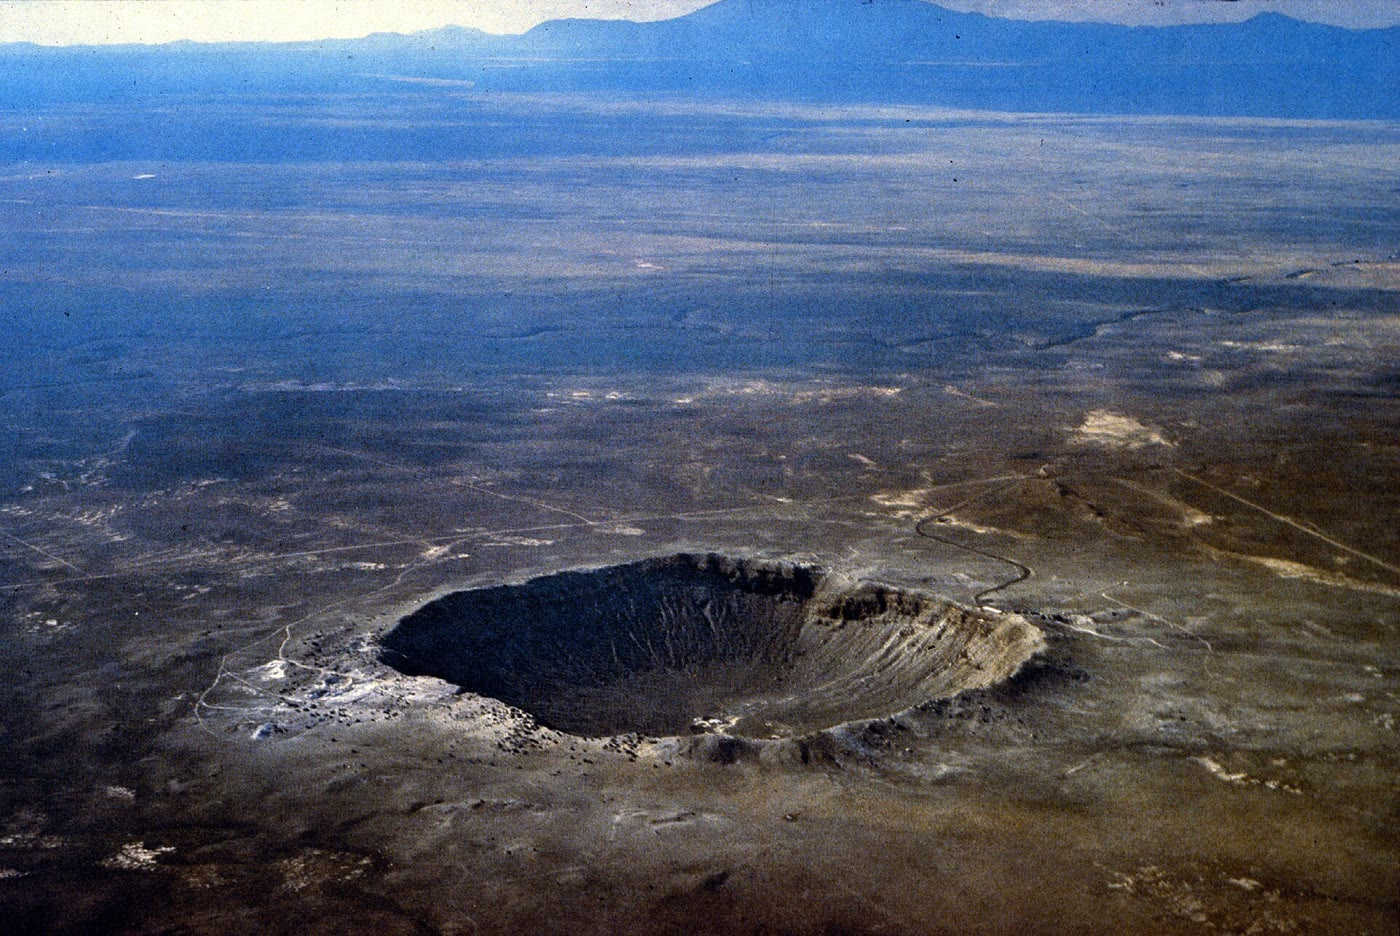
\includegraphics[width=0.66\linewidth]{images/book5/b3-barringer-crater.jpg}
\par\smallskip{\small Barringer Meteor Crater, Arizona, een \omterm{def:b3:planetary-interiors-surfaces:crater-morphology}{eenvoudige krater}
\qty{1.2}{km} breed, ongeveer 50\,000 jaar geleden gevormd door een ijzermeteoriet van
ongeveer \qty{30}{m} breed; de rand steekt boven het plateau uit en het \omterm{def:b3:planetary-interiors-surfaces:crater-morphology}{ejectadeken}
verspreidt zich eromheen. Luchtfoto, USGS/D.~Roddy, publiek
domein.}\label{fig:b3:planetary-interiors-surfaces:barringer}
\end{omfigure}
% ledger: photo:b3-barringer, french:barringer

Het uitgraven van een krater van \qty{1}{km} breed duurt ongeveer zes seconden, dat
van een krater van \qty{200}{km} breed ongeveer anderhalve minuut. Welke kratergrootte
een inslag veroorzaakt, hangt af van de energie van het projectiel, van de zwaartekracht en
van de sterkte van het gesteente; de wetten die ze met elkaar verbinden, zijn op
experimenten en explosies aangepast in de vorm van producten van dimensieloze
groepen, en worden hier aangenomen. Hun geest zit in een evenwicht van energieën.
% ledger: french:transient

\begin{proposition}[Schaling in het zwaartekrachtregime]\label{prop:b3:planetary-interiors-surfaces:scaling}
Als een vaste fractie van de inslagenergie $E$ het uitgegraven gesteente met
dichtheid $\rho$ tegen de zwaartekracht $g$ in optilt, groeit de diameter van de krater als
\[
  D \propto \left(\frac{E}{\rho g}\right)^{1/4} .
\]
\end{proposition}

\begin{proof}
Het uitgegraven volume schaalt met $D^3$, de massa ervan met $\rho D^3$, en het wordt
over een hoogte van de orde $D$ opgetild: de arbeid is van de orde $\rho g D^4$, wat
evenredig is met $E$.
\end{proof}

Een deel van de energie gaat op aan warmte, smelten en het breken van gesteente, zodat
de werkelijke wetten tussen deze en eenvoudiger regels in liggen: een tabel die voor de
Aarde vaak wordt aangehaald, geeft een krater die twintig keer zo breed is als het stenen
projectiel. De zwaartekracht bepaalt ook waar een krater ophoudt eenvoudig te zijn. De
wanden van de tijdelijke kom storten in wanneer het gewicht van het gesteente dat ze
dragen, van de orde $\rho g D/3$, de sterkte van het gesteente overschrijdt, zodat de
overgangsdiameter varieert als $1/g$: ongeveer \qty{4}{km} in kristallijn gesteente en
\qty{2}{km} in sedimenten op de Aarde, ongeveer \qty{20}{km} op de Maan, waar de
zwaartekracht zes keer zwakker is.
% ledger: french:table21, french:transition, planet:Earth.gravity, planet:Moon.gravity

\section{Kraterdatering}\label{sec:b3:planetary-interiors-surfaces:dating}

Een oppervlak dat met rust wordt gelaten, verzamelt kraters in de mate waarin lichamen
erop inslaan. Door ze te tellen wordt het oppervlak gedateerd, mits de snelheid bekend
is en de kraters die van het oppervlak zelf zijn, niet van wat eronder ligt of van het
puin dat van een buurman is weggeslingerd.

\begin{definition}[Grootte--frequentieverdeling van kraters]\label{def:b3:planetary-interiors-surfaces:sfd}
De \emph{grootte--frequentieverdeling van kraters}\index{grootte--frequentieverdeling van kraters}
van een oppervlak is het aantal kraters $N(D)$ met een diameter van ten minste $D$ per
eenheid van oppervlak, als functie van $D$ (de cumulatieve verdeling), of de aantallen
geteld in klassen van diameter, meestal elk $\sqrt2$ keer zo breed als de vorige (de
incrementele verdeling).
\end{definition}

\begin{definition}[Kraterdatering; productie- en chronologiefuncties; evenwichtsdichtheid]\label{def:b3:planetary-interiors-surfaces:crater-dating}
\emph{Kraterdatering}\index{kraterdatering} is het bepalen van de ouderdom
van een oppervlak uit de dichtheid van zijn kraters. De
\emph{kraterproductiefunctie}\index{kraterproductiefunctie} is de vorm van de
grootte--frequentieverdeling van de kraters die een oppervlak verwerft, $F(D) =
N(D)/N(\qty{1}{km})$, aangenomen dat die op elke ouderdom dezelfde is. De
\emph{kraterchronologiefunctie}\index{kraterchronologiefunctie} $N_1(T)$ is het
aantal kraters van \qty{1}{km} en groter per eenheid van oppervlak dat zich in een
tijd $T$ heeft opgehoopt. Een oppervlak bevindt zich op de
\emph{evenwichtsdichtheid van kraters}\index{evenwichtsdichtheid van kraters} voor kraters van een
gegeven grootte wanneer elke nieuwe krater gemiddeld evenveel oude wegvaagt als hij
toevoegt: hun aantal neemt dan niet meer toe.
\end{definition}

De modelouderdom van een oppervlak volgt uit één telling: $N(D)$ gemeten bij een willekeurige
$D$ geeft $N_1 = N(D)/F(D)$, en $T$ lost $N_1(T) = N_1$ op. De lijnen
$N(D) = N_1(T)F(D)$ voor vaste $T$ heten isochronen. Voor Mars wordt een
veel gebruikte productiefunctie is een polynoom van graad~11 in $\log_{10}D$, en
de chronologiefunctie heeft de vorm
\[
  N_1(T) = a\left(e^{bT} - 1\right) + cT , \qquad
  a = \qty{3.22e-14}{km^{-2}}, \ b = \qty{6.93}{Ga^{-1}}, \
  c = \qty{4.875e-4}{km^{-2}.Ga^{-1}} ,
\]
lineair over de laatste drie miljard jaar, steil exponentieel daarvoor. De
functie van de Maan heeft dezelfde vorm met $a = \num{5.44e-14}$ en $c =
\num{8.38e-4}$. Zij is gefit op de ouderdommen van de landingsplaatsen van Apollo en Luna;
die van Mars is die van de Maan, geschaald met een schatting van de verhouding van de
kratervormingssnelheden op Mars en op de Maan.
% ledger: craterstats:mars-pf, craterstats:mars-cf, craterstats:moon-cf, marchi:neukum

\begin{omfigure}
\centering
\begin{tikzpicture}
\begin{groupplot}[group style={group size=2 by 1, horizontal sep=1.6cm},
  width=0.48\linewidth, height=0.46\linewidth,
  tick label style={font=\scriptsize}, label style={font=\small}, title style={font=\small}]
\nextgroupplot[title={isochronen op Mars}, xmode=log, ymode=log, xmin=0.1, xmax=100,
  ymin=1e-8, ymax=100, xlabel={kraterdiameter $D$ (\unit{km})},
  ylabel={$N(D)$, kraters $\geq D$ per \unit{km^2}},
  xtick={0.1,1,10,100}, xticklabels={0.1,1,10,100},
  ytick={1e-8,1e-6,1e-4,1e-2,1}]
\addplot[thick, black!50, dashed] table[x=D, y=eq] {figdata/out/bachelor-3-crater_sfd-iso.dat};
\addplot[omDef] table[x=D, y=N_0.1] {figdata/out/bachelor-3-crater_sfd-iso.dat};
\addplot[omDef] table[x=D, y=N_1] {figdata/out/bachelor-3-crater_sfd-iso.dat};
\addplot[omDef] table[x=D, y=N_3.5] {figdata/out/bachelor-3-crater_sfd-iso.dat};
\addplot[red!70!black, thick] table[x=D, y=N_4] {figdata/out/bachelor-3-crater_sfd-iso.dat};
\node[font=\tiny, omDef, anchor=north east] at (axis cs:0.75,8e-6) {0.1~Ga};
\node[font=\tiny, omDef, anchor=north east] at (axis cs:2.6,1e-5) {1~Ga};
\node[font=\tiny, omDef, anchor=north east] at (axis cs:9,3.5e-5) {3.5~Ga};
\node[font=\tiny, red!70!black, anchor=north east] at (axis cs:45,2.5e-5) {4~Ga};
\node[font=\tiny, black!60, anchor=south, rotate=-30] at (axis cs:25,3.5e-4) {evenwicht};
\nextgroupplot[title={chronologiefuncties}, ymode=log, xmin=0, xmax=4.5,
  ymin=1e-5, ymax=0.3, xlabel={ouderdom $T$ (\unit{Ga})}, ylabel={$N_1$ per \unit{km^2}},
  legend style={font=\scriptsize, at={(0.03,0.97)}, anchor=north west}]
\addplot[thick, red!70!black] table[x=T, y=mars] {figdata/out/bachelor-3-crater_sfd-chron.dat};
\addlegendentry{Mars}
\addplot[thick, black!60, dashed] table[x=T, y=moon] {figdata/out/bachelor-3-crater_sfd-chron.dat};
\addlegendentry{Maan}
\end{groupplot}
\end{tikzpicture}
\par\smallskip{\small Links: isochronen van Mars, de cumulatieve dichtheden van
kraters op oppervlakken van 0.1, 1, 3.5 en 4 miljard jaar oud, met de
evenwichtsdichtheid (gestippeld), die elke telling begrenst: op een oppervlak van 4
miljard jaar oud zijn de kraters kleiner dan ongeveer \qty{0.7}{km} in evenwicht en
geven de ouderdom niet meer aan. Rechts: de chronologiefuncties van Mars en van de Maan,
het aantal kraters van \qty{1}{km} en groter per vierkante kilometer tegen de
ouderdom van
het oppervlak.}\label{fig:b3:planetary-interiors-surfaces:sfd}
\end{omfigure}
% ledger: craterstats:mars-pf, craterstats:mars-cf, craterstats:moon-cf, craterstats:equilibrium

Kraters worden willekeurig en onafhankelijk van elkaar getroffen, zodat het aantal
$n$ dat op een oppervlak wordt gevonden, is een Poissonvariabele.

\begin{proposition}[Telfout van een modelouderdom]\label{prop:b3:planetary-interiors-surfaces:poisson}
Als $n$ kraters op een oppervlak $A$ worden geteld, heeft de dichtheid $N = n/A$ de
standaarddeviatie $\sqrt n/A$, een relatieve fout $1/\sqrt n$, en de
modelouderdom de standaarddeviatie
\[
  \sigma_T = \frac{N_1(T)}{\sqrt n\,N_1'(T)} .
\]
\end{proposition}

\begin{proof}
Een Poissonvariabele met verwachtingswaarde $\lambda$ heeft variantie $\lambda$, geschat door
$n$. De ouderdom is $T = N_1^{-1}(N_1)$; in eerste orde geldt $\sigma_T =
\sigma_{N_1}/N_1'(T)$, en $\sigma_{N_1} = N_1/\sqrt n$.
\end{proof}

De relatieve fout van de telling alleen bedraagt tien procent bij honderd
kraters. Op een jong oppervlak, waar $N_1$ lineair is, erft de ouderdom die fout:
$\sigma_T/T = 1/\sqrt n$. Op een oud oppervlak verkleint de steile functie haar, met
een factor zes bij \qty{3.8}{Ga} (\cref{exo:b3:planetary-interiors-surfaces:11});
de modelouderdommen van oude oppervlakken worden dan juist beperkt door de kalibratie
van de functie zelf. Twee verdere grenzen beperken een telling. Kleine kraters verzadigen:
op de oudste oppervlakken staan kraters kleiner dan ongeveer \qty{0.7}{km} op de
evenwichtsdichtheid en registreren de tijd niet langer. En een oppervlak kan worden
vernieuwd zonder te worden uitgewist: een lavastroom die kleine kraters bedekt maar niet de
randen van grote, laat een verdeling achter met een knik, oud bij grote $D$ en
jong bij kleine $D$. De knik dateert de \omterm{def:b3:planetary-interiors-surfaces:resurfacing}{oppervlaktevernieuwing}.
% ledger: craterstats:equilibrium

\begin{definition}[Oppervlaktevernieuwing]\label{def:b3:planetary-interiors-surfaces:resurfacing}
\emph{Oppervlaktevernieuwing}\index{oppervlaktevernieuwing} is de vernieuwing van een planetair
oppervlak, door lava, sediment, ijs of vervorming, die de kraters verwijdert of bedekt en
zijn kraterklok terugzet.
\end{definition}

\section{Vulkanisme en tektoniek buiten de Aarde}\label{sec:b3:planetary-interiors-surfaces:volcanism}

Elke terrestrische planeet verliest zijn interne warmte via zijn lithosfeer.
De Aarde doet dat met bewegende platen; de andere doen het anders.

\begin{definition}[Stagnant deksel]\label{def:b3:planetary-interiors-surfaces:stagnant-lid}
Een planeet heeft een \emph{stagnant deksel}\index{stagnant deksel} wanneer zijn lithosfeer een
enkele starre schil is die niet deelneemt aan de convectie van de
mantel eronder: warmte gaat er doorheen door conductie en door het magma dat er doorheen stijgt.
Op een planeet met een mobiel deksel, zoals de Aarde, is de lithosfeer
opgebroken in platen die terugzinken in de mantel.
\end{definition}

\begin{definition}[Warmtepijpvulkanisme]\label{def:b3:planetary-interiors-surfaces:heat-pipe}
\emph{Warmtepijpvulkanisme}\index{warmtepijpvulkanisme} is het verlies van de interne warmte van een
planeet vooral door magma dat door smalle kanalen omhoog stijgt en aan het
oppervlak uitbarst, waar de lava's afkoelen en door latere lava's worden bedekt:
de lithosfeer wordt van boven opgebouwd en koud naar beneden gevoerd.
\end{definition}

\begin{omfigure}
\centering
\begin{tikzpicture}[x=0.5cm, y=0.5cm, font=\scriptsize, >=stealth]
\foreach \dx/\name in {0/mobiel deksel, 9.5/stagnant deksel, 19/warmtepijp} {
  \begin{scope}[xshift=\dx*0.5cm]
  \fill[orange!15] (0,0) rectangle (8,4);
  \node[anchor=south] at (4,5.6) {\name};
  \end{scope}}
% mobile lid: plates, ridge, slab
\fill[omDef!35] (0,4) rectangle (3.9,4.8);
\fill[omDef!35] (4.1,4) rectangle (6.2,4.8);
\fill[omDef!35] (6.2,4.8) -- (7.6,1.6) -- (6.9,1.4) -- (5.5,4.0) -- cycle;
\fill[omDef!35] (6.55,4) rectangle (8,4.8);
\draw[->, thick] (3.6,5.1) -- (1.6,5.1); \draw[->, thick] (4.4,5.1) -- (6.0,5.1);
\draw[->, red!70!black] (4,1.0) -- (4,3.6);
\draw[black!60, ->] (2.0,3.4) arc (90:270:1.0 and 1.2);
\node[anchor=north] at (4,-0.2) {platen zinken};
% stagnant lid
\begin{scope}[xshift=4.75cm]
\fill[omDef!35] (0,3.2) rectangle (8,4.8);
\draw[black!60, ->] (2.4,3.0) arc (90:270:1.2 and 1.2);
\draw[black!60, ->] (5.6,0.6) arc (-90:90:1.2 and 1.2);
\fill[red!70!black] (3.9,3.2) rectangle (4.1,4.8);
\fill[red!70!black] (3.0,4.8) -- (4,5.4) -- (5.0,4.8) -- cycle;
\node[anchor=north] at (4,-0.2) {één dikke schil};
\end{scope}
% heat pipe
\begin{scope}[xshift=9.5cm]
\fill[omDef!35] (0,1.0) rectangle (8,4.8);
\foreach \x in {1.5,4,6.5} {\fill[red!70!black] (\x-0.1,1.0) rectangle (\x+0.1,4.8);
  \fill[red!70!black] (\x-0.6,4.8) -- (\x,5.2) -- (\x+0.6,4.8) -- cycle;}
\draw[->, thick] (2.75,4.3) -- (2.75,1.6); \draw[->, thick] (5.25,4.3) -- (5.25,1.6);
\node[anchor=north] at (4,-0.2) {lava's bedekt, deksel koud};
\end{scope}
\end{tikzpicture}
\par\smallskip{\small Drie manieren om warmte te verliezen (schematisch). Links: een
mobiel deksel, platen die bij ruggen worden gevormd en bij troggen wegzinken, zoals op de
Aarde. Midden: een \omterm{def:b3:planetary-interiors-surfaces:stagnant-lid}{stagnant deksel}, één starre schil boven de convecterende mantel,
doorkruist door het magma van enkele langlevende vulkanen. Rechts: warmtepijpen,
magma dat door smalle kanalen door een dikke koude lithosfeer omhoog stijgt, waarbij de lava's
door latere lava's worden bedekt en
naar beneden worden gevoerd.}\label{fig:b3:planetary-interiors-surfaces:lids}
\end{omfigure}

Mars heeft een \omterm{def:b3:planetary-interiors-surfaces:stagnant-lid}{stagnant deksel}. Zonder platen die hen wegvoeren van hun
bronnen, groeiden zijn vulkanen lange tijd op hun plaats boven de Tharsis-
bult. Olympus Mons, de grootste bekende vulkaan in het Zonnestelsel, torent
\qty{27}{km} hoog op een basis van meer dan \qty{600}{km} breed, omringd door een
steilrand tot \qty{6}{km} hoog; de drie nabijgelegen Tharsis Montes zijn elk 350
tot \qty{400}{km} breed. Een belasting zo groot buigt de lithosfeer, en de
breedte van de geul die ze uitgraaft meet, zoals op de Aarde, de elastische dikte
van het deksel.
% ledger: nasa:olympus-mons

\begin{omfigure}
\centering
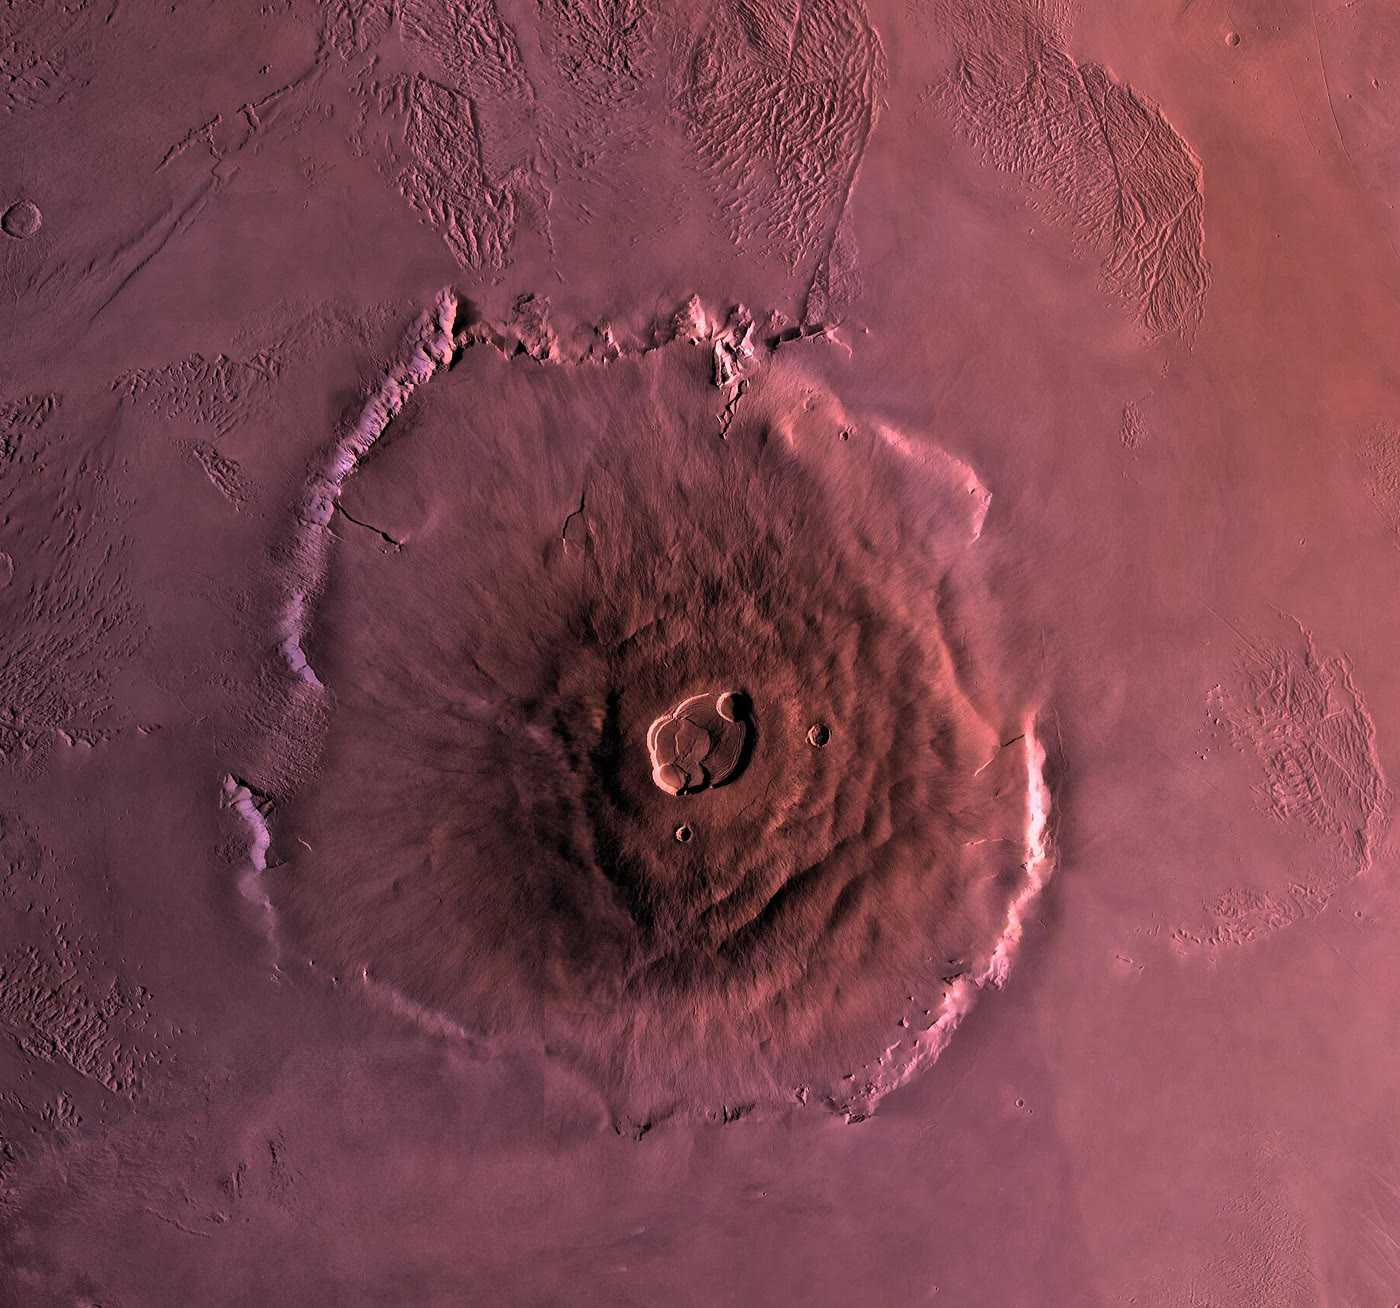
\includegraphics[width=0.48\linewidth]{images/book5/b3-olympus-mons.jpg}
\par\smallskip{\small Olympus Mons op Mars, een mozaïek van beelden van de
Viking-banen: de topcaldera's in het midden, de flanken van lavastromen en de
steilrand die de voet omringt, ongeveer \qty{600}{km} breed.
NASA/JPL/USGS, publiek domein.}\label{fig:b3:planetary-interiors-surfaces:olympus}
\end{omfigure}
% ledger: photo:b3-olympus-mons, nasa:olympus-mons

Venus, in grootte de tweelingzus van de Aarde, heeft verreweg de minste inslagkraters van
elke rotsplaneet behalve de Aarde. Zijn oppervlaktekenmerken kunnen gemiddeld zo jong zijn als
150 miljoen jaar, met tussenliggende oudere plekken:
vulkanisme en vervorming hebben het grootste deel van zijn oppervlak vernieuwd, misschien stuk voor stuk
over een lange tijd, misschien sneller. Venus heeft duizenden vulkanen en geen teken van
bewegende platen.
% ledger: nasa:venus-surface, planet:Venus.diameter, planet:Earth.diameter

Io, de binnenste grote maan van Jupiter, verliest meer dan
\qty{2.5}{W.m^{-2}} via zijn oppervlak, ongeveer 27 keer het gemiddelde van de Aarde
van \qty{0.092}{W.m^{-2}}. Zijn warmte is niet die van radioactiviteit: zij wordt
veroorzaakt door de getijden.
% ledger: veeder:io-heat, dd10:split

\begin{definition}[Getijverwarming]\label{def:b3:planetary-interiors-surfaces:tidal-heating}
\emph{Getijverwarming}\index{getijverwarming} is de warmte die binnenin een
lichaam wordt opgewekt door de wrijving van de vervorming die een wisselend getij erop uitoefent.
Een maan in synchrone rotatie op een excentrische baan ziet het getij van zijn
planeet in sterkte veranderen en tijdens elke omloop heen en weer zwaaien.
\end{definition}

\begin{proposition}[Getijvermogen van een synchrone maan]\label{prop:b3:planetary-interiors-surfaces:tidal-power}
Een maan met straal $R$ in synchrone rotatie, op een baan met gemiddelde beweging
$n$ en kleine excentriciteit $e$, dissipeert het vermogen
\[
  \dot E = \frac{21}{2}\,\frac{k_2}{Q}\,\frac{(nR)^5}{G}\,e^2 ,
\]
waarbij $Q$ de getijkwaliteitsfactor van de maan is, zodat $k_2/Q$ het
deel van de getijvervorming meet dat als warmte verloren gaat.
\end{proposition}

De propositie wordt zonder bewijs aangenomen. Getijden die energie dissiperen maken ook
een baan cirkelvormig; die van Io blijft elliptisch, met een excentriciteit van 0.004, omdat de
precies getimede trekkrachten van Europa en Ganymedes hem verstoren, hun omloopperioden
van 1.77, 3.55 en \num{7.15}~dagen zich bijna exact verhouden als
1:2:4 (zie \cref{exo:b3:planetary-interiors-surfaces:8}). Het oppervlak van Io stijgt
en daalt met maximaal \qty{100}{m} per omloop. De vulkanen
bedekken Io met lava sneller dan er kraters op kunnen ontstaan; één model voor
hoe de warmte ontsnapt, is \omterm{def:b3:planetary-interiors-surfaces:heat-pipe}{warmtepijpvulkanisme}, dat een dikke,
koude lithosfeer onder zijn vurige oppervlak in stand zou houden.
% ledger: nasa:galilean-orbits, beuthe:tidal-power, nasa:io-orbit, nasa:io-facts

\begin{definition}[Ondergrondse oceaan]\label{def:b3:planetary-interiors-surfaces:ocean-world}
Een \emph{ondergrondse oceaan}\index{ondergrondse oceaan} is een wereldwijde laag
vloeibaar water onder de ijsschil van een maan of dwergplaneet, dat vloeibaar blijft door
getij- en radiogene warmte.
\end{definition}

\begin{definition}[Cryovulkanisme]\label{def:b3:planetary-interiors-surfaces:cryovolcanism}
\emph{Cryovulkanisme}\index{cryovulkanisme} is de uitbarsting van water, pekel
of andere vluchtige vloeistoffen en dampen, in plaats van gesmolten gesteente, op het
ijzige oppervlak van een maan of dwergplaneet.
\end{definition}

De ijsschil van Europa, gemeten door de microgolfradiometer van de ruimtesonde Juno
in het gebied waar die overheen vloog, gemiddeld ongeveer \qty{29}{km} dik;
eronder ligt een zoute oceaan die twee keer zoveel water bevat als alle
oceanen van de Aarde. Op Saturnus' maan Enceladus, slechts ongeveer \qty{500}{km}
in doorsnee, vond de ruimtesonde Cassini in 2005 straalstromen van ijskorrels en gas
die uit warme breuken nabij de zuidpool ontsnapten, met ongeveer
\qty{400}{m.s^{-1}}. Zijn zwaartekracht en de slingering van zijn rotatie tonen
dat de straalstromen putten uit een wereldwijde oceaan, onder een ijsschil van 20 tot
\qty{25}{km} dik gemiddeld en misschien slechts 1 tot \qty{5}{km} bij de
zuidpool.
% ledger: jpl:europa-shell, nasa:europa-ocean, nasa:enceladus

\section{Grote kernen en kleine}\label{sec:b3:planetary-interiors-surfaces:cores}

De vier gemeten kernen vormen een vreemde familie. Relatief ten opzichte van de straal reikt de
kern van de Aarde tot 0.55 van de weg naar het oppervlak en die van Mars 0.54; die van de
Maan 0.19; die van Mercurius 0.82. Differentiatie, in Boek~4, scheidt
metaal van silicaat binnenin elk lichaam, maar kan de verhoudingen van
metaal niet zo sterk laten verschillen. Reusachtige inslagen kunnen dat wel. De Maan wordt
gedacht te zijn ontstaan uit het puin van een botsing tussen een lichaam ter grootte van Mars en de
jonge Aarde, ongeveer 4.5 miljard jaar geleden, waarbij het metaal van het inslaande lichaam
zich bij de kern van de Aarde voegde en de Maan vooral mantelgesteente verzamelde, vandaar haar
kleine kern. Vergelijkbare inslagen kunnen een groot deel van de silicaatmantel
van Mercurius hebben weggeslagen en er de ijzerrijke planeet van hebben gemaakt waarvan de kern
het grootste deel ervan vult. De kernen leggen, net als de kraters, een geschiedenis van botsingen vast.
% ledger: data:prem, jpl:insight-interior, nasa:moon-core, agu:mercury-core, french:giant-impacts

\section{Oefeningen}

\begin{exercise}[$\star$]\label{exo:b3:planetary-interiors-surfaces:1}
Mercurius heeft een gemiddelde dichtheid van \qty{5429}{kg.m^{-3}}, een traagheidsmomentfactor
van 0.35 en een straal van \qty{2440}{km}. Met een tweelagenmodel en een
mantel van \qty{3300}{kg.m^{-3}}, bereken de relatieve straal van de kern,
de straal in kilometer en de dichtheid ervan.
\end{exercise}

\begin{exercise}[$\star$]\label{exo:b3:planetary-interiors-surfaces:2}
Een stenig projectiel met een diameter van \qty{50}{m} en een dichtheid van \qty{3500}{kg.m^{-3}},
treft de Aarde loodrecht met \qty{20}{km.s^{-1}}. Bereken de massa en
de kinetische energie ervan, in joule en in megaton explosief
($\qty{1}{Mt} = \qty{4.2e15}{J}$). Welke kraterdiameter volgt uit de regel van
twintig projectieldiameters?
\end{exercise}

\begin{exercise}[$\star$]\label{exo:b3:planetary-interiors-surfaces:3}
Op een Marsvlakte van \qty{100000}{km^2} zijn 120 kraters van \qty{1}{km} en groter
geteld. Bereken $N_1$, de relatieve fout ervan en de modelouderdom van
de vlakte met de bijbehorende fout.
\end{exercise}

\begin{exercise}[$\star$]\label{exo:b3:planetary-interiors-surfaces:4}
Io, met een straal van \qty{1821.5}{km}, verliest \qty{2.5}{W.m^{-2}}. Bereken zijn
totale warmteverlies en vergelijk het met dat van de Aarde, \qty{47}{TW}, in totaal en
per vierkante meter (\qty{0.092}{W.m^{-2}}).
\end{exercise}

\begin{exercise}[$\star\star$]\label{exo:b3:planetary-interiors-surfaces:5}
Mars heeft een massa van \qty{6.417e23}{kg} en een straal van \qty{3389.5}{km}.
(a)~Bereken de gemiddelde dichtheid, de zwaartekracht aan het oppervlak en $\rho gR$.
(b)~Behandel het als een uniforme onsamendrukbare bol met een stijfheid van
\qty{67}{GPa}, bereken het \omterm{def:b3:planetary-interiors-surfaces:love-number}{Lovegetal} $k_2$. (c)~De gemeten waarde is
$0.153 \pm 0.017$. Wat zegt de vergelijking?
\end{exercise}

\begin{exercise}[$\star\star$]\label{exo:b3:planetary-interiors-surfaces:6}
Op de Aarde ($g = \qty{9.8}{m.s^{-2}}$) ligt de overgang van eenvoudig naar
complex bij ongeveer \qty{4}{km} in kristallijn gesteente en \qty{2}{km} in
sedimenten. (a)~Neem aan dat de overgangsdiameter evenredig is met $1/g$;
voorspel die op de Maan ($g = \qty{1.62}{m.s^{-2}}$) en op Mars en Mercurius
($g = \qty{3.7}{m.s^{-2}}$); vergelijk met de \qty{20}{km} die op de Maan is waargenomen.
(b)~Als instorting begint wanneer $\rho gD/3$ de sterkte $Y$ van het gesteente overschrijdt,
welke sterkte volgt dan uit de overgang in kristallijn gesteente op de Aarde,
voor $\rho = \qty{2600}{kg.m^{-3}}$?
\end{exercise}

\begin{exercise}[$\star\star$]\label{exo:b3:planetary-interiors-surfaces:7}
Een oppervlak bevat $\num{2.0e-3}$ kraters van \qty{1}{km} en groter per
vierkante kilometer. Bepaal de modelouderdom met de \omterm{def:b3:planetary-interiors-surfaces:crater-dating}{kraterchronologiefunctie} van Mars
door de vergelijking numeriek op te lossen. Welke modelouderdom zou de maanfunctie
hebben opgeleverd, en waarom mogen de twee niet worden verwisseld?
\end{exercise}

\begin{exercise}[$\star\star$]\label{exo:b3:planetary-interiors-surfaces:8}
De omlooptijden van Io, Europa en Ganymedes zijn 1.769138, 3.551181 en
\num{7.154553}~dagen. (a)~Bereken de verhoudingen van opeenvolgende omlooptijden.
(b)~Bereken $1/P_I - 3/P_E + 2/P_G$ en geef commentaar. (c)~Waarom kunnen resonanties
een excentriciteit in stand houden die getijden anders zouden wegwerken?
\end{exercise}

\begin{exercise}[$\star\star$]\label{exo:b3:planetary-interiors-surfaces:9}
Io draait in \num{1.769138}~dagen om Jupiter met excentriciteit 0.004.
Bereken het vermogen dat de propositie over getijdenvermogen geeft per eenheid $k_2/Q$,
en de waarde van $k_2/Q$ die Io's warmteverlies
uit \cref{exo:b3:planetary-interiors-surfaces:4} zou leveren.
\end{exercise}

\begin{exercise}[$\star\star\star$]\label{exo:b3:planetary-interiors-surfaces:10}
Voor de Maan geldt $\bar\rho = \qty{3340}{kg.m^{-3}}$ en $C = 0.394$.
(a)~Toon aan dat in het tweelagenmodel $\mathrm dx^2/\mathrm dC =
\tfrac52\bar\rho/(\bar\rho - \rho_m)$ bij vaste $\rho_m$. (b)~Met de
manteldichtheid die een kern van $x = 0.19$ geeft, \qty{3288}{kg.m^{-3}},
wat zijn $x$ en $\rho_c$ wanneer $C = 0.395$, en wanneer $C = 0.393$?
(c)~Wat zegt dit over het bepalen van de grootte van een kleine kern met
het traagheidsmoment?
\end{exercise}

\begin{exercise}[$\star\star\star$]\label{exo:b3:planetary-interiors-surfaces:11}
(a)~Bereken voor 100 kraters de telfout van de modelouderdom van een
marsoppervlak van \qty{1.0}{Ga} oud en van een van \qty{3.8}{Ga} oud.
(b)~Toon aan dat op het lineaire deel van de \omterm{def:b3:planetary-interiors-surfaces:crater-dating}{kraterchronologiefunctie} $\sigma_T/T =
1/\sqrt n$. (c)~Waarom zijn de ouderdommen van oude oppervlakken dan nog onzeker?
\end{exercise}

\begin{exercise}[$\star\star\star$]\label{exo:b3:planetary-interiors-surfaces:12}
Europa, met een straal van \qty{1560.8}{km}, draait in \num{3.551181}~dagen met
excentriciteit 0.009. (a)~Neem aan dat Europa getijden dissipeert met dezelfde $k_2/Q$
als Io. Welk deel van Io's getijdenvermogen zou het opwekken, en welke warmtestroom?
(b)~Waarom is de aanname twijfelachtig voor een maan met een \omterm{def:b3:planetary-interiors-surfaces:ocean-world}{ondergrondse oceaan} onder het ijs?
\end{exercise}

\section{Probleem: Twee vlakten op Mars}

\begin{problem}[{Weekendprobleem --- de kern van Mars en de ouderdommen van twee
verzonnen lavavlakten}]
\label{pb:b3:planetary-interiors-surfaces:1}
Mars heeft een massa van \qty{6.4169e23}{kg}, een straal van \qty{3389.5}{km} en een
traagheidsmomentfactor van 0.366. Twee verzonnen vlakten, A en B, liggen op zijn
vulkanische provincies; hun kraters zijn geteld op beelden in klassen
van $\sqrt2$ breed.

\medskip\noindent\textbf{Deel I --- De kern.}
\begin{enumerate}
\item Bereken de gemiddelde dichtheid van Mars.
\item Bereken met een tweelagenmodel en een mantel van \qty{3500}{kg.m^{-3}}
  de relatieve straal van de kern, de straal in kilometers en de
  dichtheid ervan.
\item InSight mat een kernstraal van \qty{1830}{km}. Welke manteldichtheid
  en kerndichtheid vereist het tweelagenmodel dan?
\item Vergelijk die kerndichtheid met de dichtheid van de buitenkern van de Aarde
  vlak onder de bovenkant, \qty{9900}{kg.m^{-3}} in het referentiemodel van de aarde,
  en zeg waarom voor Mars een lagere waarde wordt verwacht, en wat het verder
  suggereert.
\item Het \omterm{def:b3:planetary-interiors-surfaces:love-number}{Lovegetal} van Mars voor een homogene bol met een stijfheid van
  \qty{67}{GPa} is 0.109; het gemeten is 0.153. Welke waarneming kwam
  eerst, en wat zei die al over de kern?
\item De korst van Mars is 20 tot \qty{37}{km} dik. Welk deel van het
  volume van de planeet beslaat ze? Was het juist om haar te negeren?
\end{enumerate}

\medskip\noindent\textbf{Deel II --- De tellingen op vlakte A.} Vlakte A
beslaat \qty{80000}{km^2}. De kraters, per klasse van diameter (km):
\begin{center}
\small
\begin{tabular}{lccccccccc}
\hline
klasse & 1--1.41 & 1.41--2 & 2--2.83 & 2.83--4 & 4--5.66 & 5.66--8 & 8--11.3 & 11.3--16 & 16--22.6 \\
\hline
vlakte A & 38 & 6 & 5 & 3 & 0 & 0 & 0 & 1 & 1 \\
vlakte B & 48 & 8 & 31 & 12 & 7 & 2 & 0 & 2 & 2 \\
\hline
\end{tabular}
\end{center}
\begin{enumerate}[resume]
\item Bereken de cumulatieve tellingen van vlakte A, vanaf \qty{1}{km} omhoog.
\item Bereken $N(\qty{1}{km})$ per vierkante kilometer en de
  bijbehorende standaarddeviatie.
\item De productiefunctie geeft $F(\qty{2}{km}) = 0.147$ en
  $F(\qty{1.41}{km}) = 0.355$. Zijn de tellingen bij 1.41 en \qty{2}{km}
  in overeenstemming met de vorm van de productiefunctie?
\item Ligt vlakte A ergens in de buurt van de \omterm{def:b3:planetary-interiors-surfaces:crater-dating}{evenwichtsdichtheid van kraters},
  \qty{0.072}{km^{-2}} bij \qty{1}{km}?
\item Waarom zijn de klassen gekozen met een breedte van $\sqrt2$?
\item Clusters en kettingen van kleine kraters worden buiten een telling gelaten. Waarom?
\end{enumerate}

\medskip\noindent\textbf{Deel III --- Modelouderdommen.} Gebruik de
chronologiefunctie van Mars.
\begin{enumerate}[resume]
\item Bereken de modelouderdom van vlakte A. Controleer dat de exponentiële term
  verwaarloosd mag worden.
\item Bereken de telfout daarvan.
\item Welke ouderdom zou de maankronologie hebben opgeleverd?
\item Vlakte B beslaat \qty{120000}{km^2}. Bereken met de kraters van \qty{2}{km}
  en groter eerst $N(\qty{2}{km})$, dan $N_1$ en daarna de modelouderdom door
  de vergelijking numeriek op te lossen.
\item Bereken de telfout van die ouderdom.
\item Vergelijk de relatieve fouten van de twee ouderdommen en verklaar het
  verschil.
\end{enumerate}

\medskip\noindent\textbf{Deel IV --- De begraven kraters van vlakte B.}
\begin{enumerate}[resume]
\item Hoeveel kraters tussen 1 en \qty{2}{km} zou vlakte B moeten bevatten als
  het hele oppervlak de ouderdom van vraag~16 had? Hoeveel bevat zij er werkelijk?
\item Neem aan dat lava elke krater kleiner dan \qty{2}{km} begroef op een
  moment $T_r$ en de grotere spaarde. Bereken $T_r$ uit de kraters van
  \num{1}--\qty{2}{km}.
\item Bereken de telfout van $T_r$.
\item Neem aan dat een verse \omterm{def:b3:planetary-interiors-surfaces:crater-morphology}{eenvoudige krater} op Mars half zo diep is als
  hij breed is (een aanname van dit vraagstuk). Hoe dik moet de lava zijn om
  een krater van \qty{2}{km} te begraven, en waarom zijn de grotere nog zichtbaar?
\item Kunnen de lava van vlakte B en die van vlakte A tot dezelfde episode
  van vulkanisme behoren?
\item Geef de modelouderdom van vlakte A, in miljard jaar, met twee
  significante cijfers.
\end{enumerate}
\end{problem}
% ledger: nasa:mars, jpl:insight-interior, yoder:mars-k2, data:prem, craterstats:mars-pf, craterstats:mars-cf, craterstats:moon-cf, craterstats:equilibrium
